\chapter{Análisis y selección de \emph{hardware} y \emph{software}}
\label{ch:seleccion_hardware_software}

En este capítulo se expone el análisis técnico, normativo y económico para la definición de la plataforma de adquisición de datos y el entorno de software aplicados a la modernización del sistema de medición del ensayo de impulso del Laboratorio de Alta Tensión. Se analiza el estado actual del equipamiento del laboratorio, se evalúa el sistema comercial de referencia internacional, se comparan los instrumentos disponibles, y se fundamenta la selección final del hardware de medición y de la arquitectura de software desarrollada.

\section{Análisis del equipamiento de referencia}
\label{sec:estado_actual_owon}
\vspace{3\baselineskip}

Como se mencionó antes, el LAT contaba con el osciloscopio \emph{Nicolet PowerPro 610} (figura \ref{fig:nicolet_610}), que podía caracterizar impulsos tipo rayo. A continuación, la tabla \ref{tab:nicolet_especificaciones} detalla sus especificaciones técnicas, las cuales sirvieron como punto de partida para la búsqueda de un sustituto.

\vspace{3\baselineskip}
\begin{figure}[H]
    \centering
    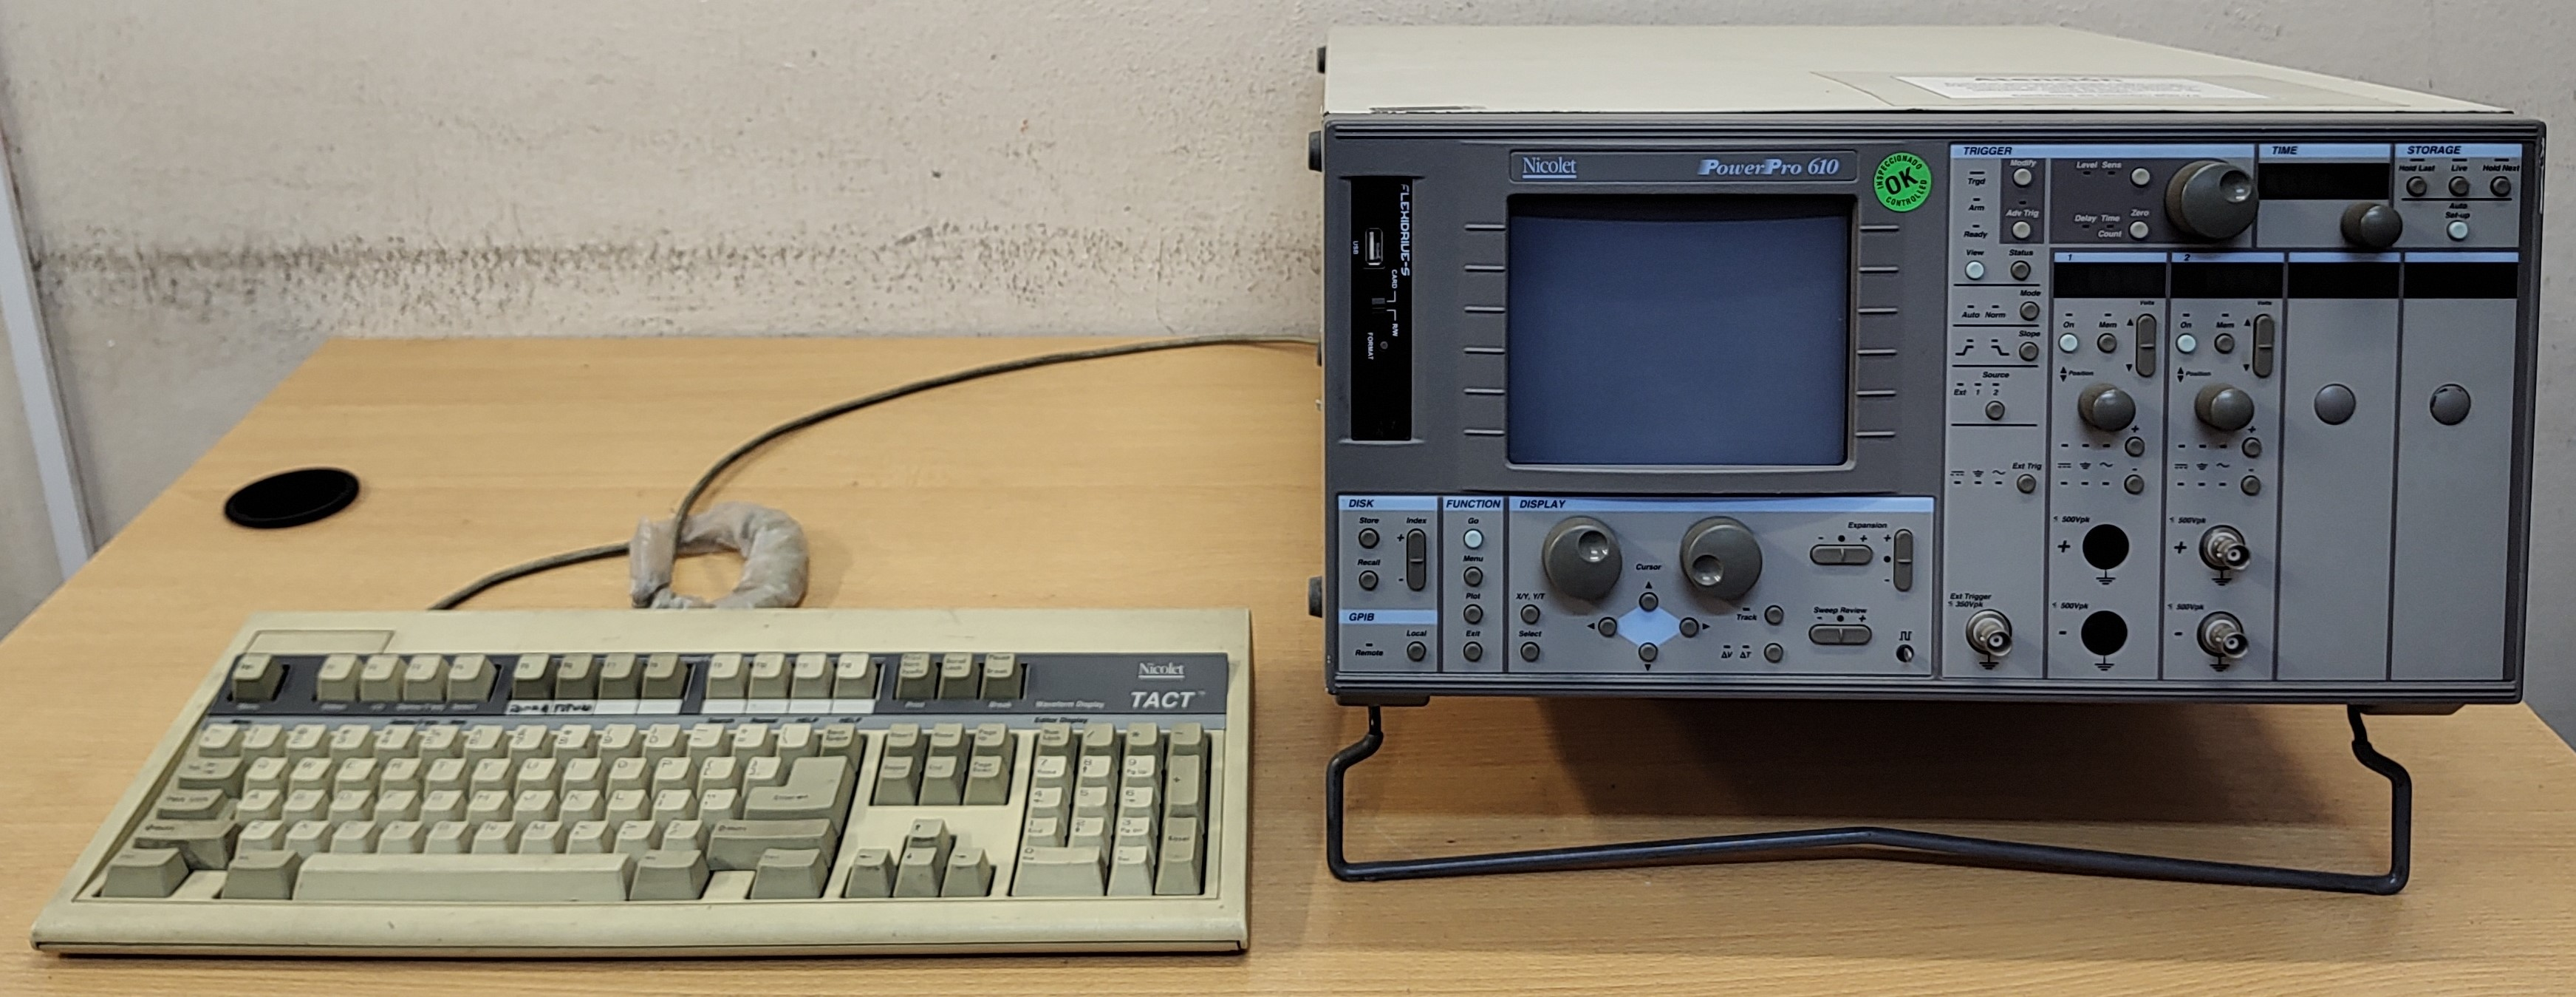
\includegraphics[width=\textwidth]{img/osciloscopios/nicolet_610.jpg}
    \caption{Osciloscopio Nicolet PowerPro 610. Fuente: Propia.}
    \label{fig:nicolet_610}
\end{figure}
\vspace{3\baselineskip}

\vspace{3\baselineskip}
\begin{table}[H]
    \centering
    \caption{Características técnicas del osciloscopio Nicolet PowerPro 610.}
    \label{tab:nicolet_especificaciones}
    \begin{tabular}{ll}
        \toprule
        \textbf{Parámetro técnico} & \textbf{Valor nominal} \\ \midrule
        Ancho de banda & \qty{25}{\mega\hertz} \\ \midrule
        Tasa de muestreo máxima & \qty{75}{\mega\sample/\second} \\ \midrule
        Tensión de entrada máxima & \qty{500}{\volt} \\ \midrule
        Longitud de memoria & \num{256} k / \num{1} M \\ \midrule
        Resolución vertical & \qty{10}{bit} \\ \bottomrule
    \end{tabular}
\end{table}
\vspace{3\baselineskip}

A raíz de la salida de servicio del equipo, el laboratorio adoptó el uso del osciloscopio de uso general \emph{Owon PDS7102T} que puede verse en la figura \ref{fig:owon_pds7102t}. Bajo esta modalidad, la adquisición se realiza capturando la señal con el instrumento para efectuar posteriormente un trazado y análisis visual de los parámetros de impulso con el software propietario del equipo.

\subsection{Alternativas comerciales de referencia}
\label{subsec:alternativas_comerciales}

Para establecer la cota superior del estado del arte en la instrumentación de impulsos de alta tensión, se examinó el sistema comercial dedicado HAEFELY HiAS 744 \cite{haefely_datasheet}, que puede apreciarse en la figura \ref{fig:Haefely_HiAS744}. Este equipo representa el máximo exponente tecnológico a nivel internacional para el análisis de impulso tipo rayo de \qty[parse-numbers=false]{1,2/50}{\micro\second}, cumpliendo de manera estricta los requerimientos de las normas IEC 60060-1, IEC 60060-2 e IEC 61083-2 \cite{iec61083_2}.

\vspace{3\baselineskip}
\begin{figure}[H]
    \centering
    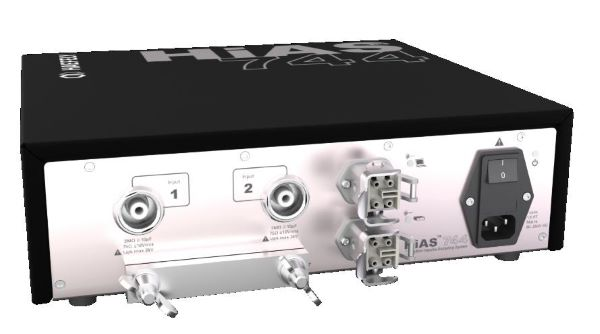
\includegraphics[width=0.2\textwidth]{img/osciloscopios/HiAS_744.jpg}
    \caption{Equipo de adquisición Haefely HiAS 744. Fuente: \cite{haefely_datasheet}.}
    \label{fig:Haefely_HiAS744}
\end{figure}
\vspace{3\baselineskip}

El sistema incorpora desacoplamiento óptico mediante enlaces de fibra óptica hacia la estación de control, logrando un aislamiento galvánico total que elimina bucles de tierra y protege al operador frente a descargas destructivas.

El producto se comercializa en tres variantes cuyas especificaciones técnicas \cite{haefely_datasheet} se resumen en la tabla \ref{tab:haefely_hias744_comparativa}, con sus costos aproximados en septiembre de 2026\footnote{El precio fue consultado al fabricante.}.

\vspace{3\baselineskip}
\begin{table}[H]
    \centering
        \caption{Especificaciones técnicas y costos de la serie HAEFELY HiAS 744.}
        \label{tab:haefely_hias744_comparativa}
        \begin{tabular}{lccc}
            \toprule
            \textbf{Parámetro técnico} & \textbf{HiAS 744} & \textbf{HiAS 744-S} & \textbf{HiAS 744-REF} \\ \midrule
            Resolución vertical & \qty{11}{bit} (\qty{0,05}{\percent}) & \qty{16}{bit} (\qty{0,0015}{\percent}) & \qty{16}{bit} (\qty{0,0015}{\percent}) \\ \midrule
            Tasa de muestreo máxima & \qty{125}{\mega\sample/\second} & \qty{250}{\mega\sample/\second} & \qty{250}{\mega\sample/\second} \\ \midrule
            Ancho de banda & $\ge \qty{50}{\mega\hertz}$ & $\ge \qty{100}{\mega\hertz}$ & $\ge \qty{100}{\mega\hertz}$ \\ \midrule
            Profundidad de memoria & \num{2} Mpts & \num{2} Mpts & \num{2} Mpts \\ \midrule
            Aislamiento e interfaz de datos & Fibra óptica & Fibra óptica & Fibra óptica \\ \midrule
            Calibración metrológica & De fábrica & De fábrica & ISO/IEC 17025 \\ \midrule
            Costo & \qty{59000}{USD} & \qty{75000}{USD} & No especificado \\ \bottomrule
        \end{tabular}
\end{table}
\vspace{3\baselineskip}

\subsection{Evaluación de equipos disponibles}
\label{subsec:comparativa_osciloscopios_laboratorio}

Frente a la restricción presupuestaria que impide adquirir un analizador comercial dedicado como el HAEFELY HiAS 744, se procedió a evaluar los cuatro osciloscopios de propósito general disponibles en el laboratorio: Owon PDS7102T (figura \ref{fig:owon_pds7102t}), GW Instek GDS-1022 (figura \ref{fig:gwinstek_gds_1022}), GW Instek GDS-1102A-U (figura \ref{fig:gwinstek_gds1102au}) y Keysight DSO1052B (figura \ref{fig:keysight_dso1052b}).

Para garantizar la captura adecuada de señales con tiempo de frente de impulso $T_1 = \qty{1,2}{\micro\second}$, la tasa de muestreo debe ser superior a \qty{2}{\mega\sample/\second}.

\vspace{3\baselineskip}
\begin{figure}[H]
    \centering
    \begin{subfigure}[b]{0.45\linewidth}
        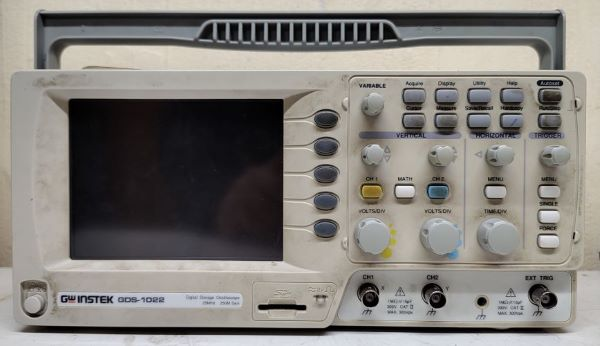
\includegraphics[width=\linewidth]{img/montaje_ensayo/gwinstek_gds_1022.jpg}
        \caption{GW Iinstek GDS1022.}
        \label{fig:gwinstek_gds_1022}
    \end{subfigure}
    \begin{subfigure}[b]{0.45\linewidth}
        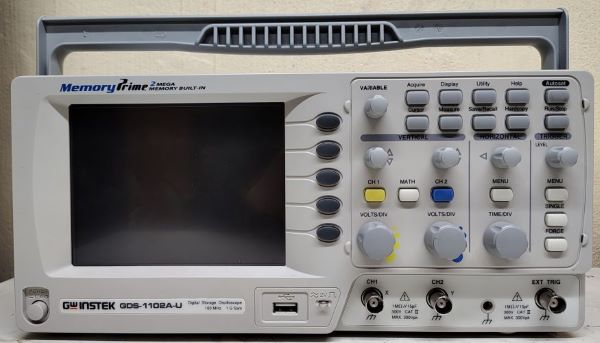
\includegraphics[width=\linewidth]{img/osciloscopios/gwinstek_gds1102au.jpg}
        \caption{GW Iinstek GDS1102A-U.}
        \label{fig:gwinstek_gds1102au}
    \end{subfigure}
        \begin{subfigure}[b]{0.45\linewidth}
        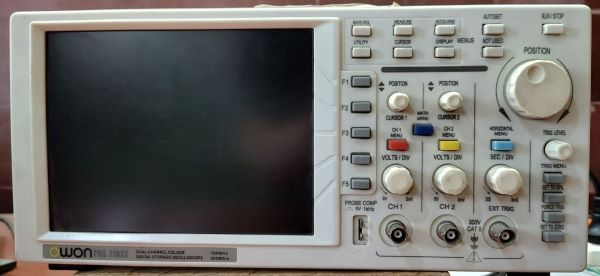
\includegraphics[width=\linewidth]{img/osciloscopios/owon_pds7102t.jpg}
        \caption{Owon PDS7102T.}
        \label{fig:owon_pds7102t}
    \end{subfigure}
    \begin{subfigure}[b]{0.45\linewidth}
        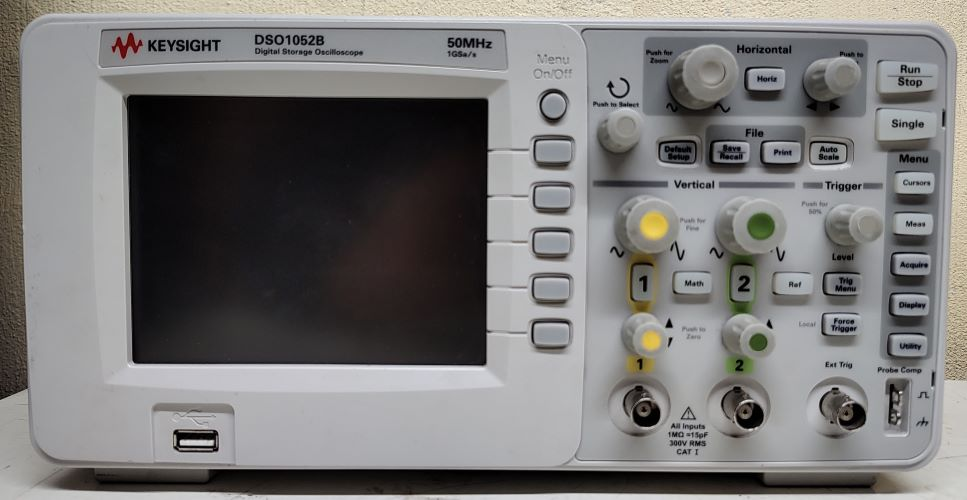
\includegraphics[width=\linewidth]{img/osciloscopios/keysight_dso1052b.jpg}
        \caption{Keysight DSO1052B.}
        \label{fig:keysight_dso1052b}
    \end{subfigure}
    \caption{Osciloscopios disponibles. Fuente: Propia.}
    \label{fig:osciloscopios_disponibles}
\end{figure}
\vspace{3\baselineskip}


La selección definitiva del instrumento se realizó con base en cuatro criterios fundamentales: ancho de banda y tasa de muestreo, longitud de memoria de registro, documentación disponible de comandos SCPI y compatibilidad con VISA, buscando que sean los más próximos al equipo de referencia de la tabla (\ref{tab:haefely_hias744_comparativa}). A continuación, la tabla \ref{tab:comparativa_osciloscopios} muestra la evaluación técnica comparativa entre las alternativas disponibles, donde debe considerarse que todas las opciones tienen resolución de \qty{8}{bit}.

\vspace{3\baselineskip}
\begin{table}[H]
    \centering
    \begin{small}
        \caption{Comparativa técnica de osciloscopios disponibles en el laboratorio.}
        \label{tab:comparativa_osciloscopios}
        \begin{tabular}{cccccc}
            \toprule
            \textbf{Equipo} & \textbf{Ancho de banda} & \textbf{Tasa de muestreo} & \textbf{SCPI} & \textbf{VISA} \\ \midrule
            Owon PDS7102T & \qty{100}{\mega\hertz} & \qty{500}{\mega\sample/\second} & No & No \\ \midrule
            GW Instek GDS-1022 & \qty{25}{\mega\hertz} & \qty{250}{\mega\sample/\second} & Sí & Sí \\ \midrule
            GW Instek GDS-1102A-U & \qty{100}{\mega\hertz} & \qty{1}{\giga\sample/\second} & Sí & Sí \\ \midrule
            Keysight DSO1052B & \qty{100}{\mega\hertz} & \qty{1}{\giga\sample/\second} & No & No \\ \bottomrule
        \end{tabular}
    \end{small}
\end{table}
\vspace{3\baselineskip}

Del análisis realizado se determina que las alternativas Keysight DSO1052B y Owon PDS7102T debieron ser descartadas, debido a la ausencia de manuales de programación de comandos SCPI e incompatibilidad con la arquitectura VISA, lo que impide su integración automatizada con un entorno de software externo.

Entre los osciloscopios del fabricante GW Instek, el modelo GDS-1102A-U fue seleccionado frente al modelo GDS-1022, debido a su mayor ancho de banda y su superior frecuencia de muestreo máxima, permitiendo un registro adecuado de impulsos de interés. La tabla \ref{tab:gwinstek_especificaciones} sintetiza las características del modelo seleccionado.

\vspace{3\baselineskip}
\begin{table}[H]
    \centering
    \caption{Especificaciones técnicas del osciloscopio GW Instek GDS-1102A-U.}
    \label{tab:gwinstek_especificaciones}
    \begin{tabular}{ll}
        \toprule
        \textbf{Parámetro técnico} & \textbf{Valor nominal} \\ \midrule
        Ancho de banda & \qty{100}{\mega\hertz} \\ \midrule
        Tasa de muestreo máxima & \qty{1}{\giga\sample/\second} \\ \midrule
        Tensión de entrada máxima & \qty{300}{\volt} \\ \midrule
        Longitud de memoria & \num{4} k / \num{2} M pts \\ \midrule
        Resolución vertical & \qty{8}{bit} \\ \bottomrule
    \end{tabular}
\end{table}
\vspace{3\baselineskip}

\section{Análisis de alternativas de \emph{software}}
\label{sec:comparativa_software}
\vspace{3\baselineskip}

Una vez definido el hardware de adquisición, se evaluaron las alternativas para el desarrollo del entorno de automatización, procesamiento digital de señales y generación de reportes. Se contrapuso el uso del software comercial \emph{National Instruments LabVIEW} frente al ecosistema del lenguaje de programación \emph{Python}~\cite{python}.

Ambas plataformas cuentan con capacidad técnica para lograr la adquisición remota de datos vía protocolos VISA/SCPI, y procesar las ondas registradas. No obstante, una licencia comercial perpetua de desarrollo de \emph{LabVIEW} implica un costo de aproximadamente \qty{1100}{USD}\footnote{El precio fue consultado al fabricante.}. Asimismo, \emph{LabVIEW} opera como un entorno cerrado ("caja negra"), dificultando la auditoría interna de sus algoritmos matemáticos.

Por el contrario, la solución basada en \emph{Python} emplea bibliotecas de código abierto (\emph{open source}) bajo licencias permisivas (BSD, MIT y LGPL) como PyVISA~\cite{pyvisa}, NumPy~\cite{numpy}, SciPy~\cite{scipy}, PySide6~\cite{pyside6} y h5py~\cite{h5py}. Este enfoque representa un costo económico nulo, brindando transparencia absoluta al desarrollador para auditar, verificar y adaptar los algoritmos exigidos por la norma IEC 61083-2 \cite{iec61083_2}. La tabla \ref{tab:comparativa_software_costos} expone la comparativa técnica y económica entre ambas soluciones.

\vspace{3\baselineskip}
\begin{table}[H]
    \centering
    \begin{small}
        \caption{Comparativa técnica y económica entre LabVIEW y Python.}
        \label{tab:comparativa_software_costos}
        \begin{tabular}{lcc}
            \toprule
            \textbf{Criterio de evaluación} & \textbf{NI LabVIEW} & \textbf{Ecosistema Python} \\ \midrule
            Costo de licencia & $\sim$\qty{1100}{USD} (Perpetua) & \qty{0}{USD} (Gratuito / Open Source) \\ \midrule
            Código fuente & Propietario & Accesible y auditable \\ \midrule
            Librerías de control y GUI & NI-VISA / LabVIEW GUI & PyVISA / PySide6 / Qt Designer \\ \midrule
            Procesamiento numérico & Módulos dedicados NI & NumPy / SciPy / h5py \\ \midrule
            Costo Total de Propiedad & Elevado & Nulo \\ \bottomrule
        \end{tabular}
    \end{small}
\end{table}
\vspace{3\baselineskip}

\subsection{Selección de la arquitectura}

A continuación se sintetizan las diferencias estructurales principales entre los tres patrones desarrollados en el capítulo \ref{ch:arquitectura_software}.

\vspace{3\baselineskip}
\begin{table}[H]
    \centering
    \small
    \caption{Evaluación comparativa entre patrones arquitectónicos.}
    \label{tab:comparacion_patrones}
    \begin{tabularx}{\textwidth}{>{\hsize=1.0\hsize}Y >{\hsize=1.0\hsize}Y >{\hsize=1.0\hsize}Y >{\hsize=1.0\hsize}Y}
        \toprule
        \textbf{Atributo} & \textbf{MVC} & \textbf{MVP} & \textbf{MVVM} \\
        \midrule
        \textbf{Mantenibilidad} & 
        \textbf{Media}\newline
        Cambios en el Modelo impactan directamente en la Vista. & 
        \textbf{Alta}\newline
        La lógica de presentación reside exclusivamente en el Presentador. & 
        \textbf{Muy Alta}\newline
        La interfaz declarativa y la lógica de estado están completamente separadas. \\
        \midrule
        \textbf{Prueba unitaria} & 
        \textbf{Baja}\newline
        Dificultad para aislar la Vista por su dependencia directa con el Modelo y el Controlador. & 
        \textbf{Alta}\newline
        El Presentador se prueba sustituyendo la Vista por abstracciones, sin componentes gráficos. & 
        \textbf{Muy Alta}\newline
        El VistaModelo carece de dependencias de clases gráficas. \\
        \midrule
        \textbf{Escalabilidad} & 
        \textbf{Baja}\newline
        Las dependencias cruzadas entre eventos de usuario y notificaciones del Modelo dificultan el flujo de datos. & 
        \textbf{Media}\newline
        Introduce un alto volumen de código repetitivo por la sincronización manual. & 
        \textbf{Media}\newline
        Requiere experiencia en el manejo de enlace de datos para evitar degradación de rendimiento. \\
        \midrule
        \textbf{Desacoplamiento} & 
        \textbf{Bajo}\newline
        Acoplamiento directo Vista $\rightarrow$ Modelo.\newline
        Acoplamiento bidireccional Controlador $\leftrightarrow$ Vista. & 
        \textbf{Alto}\newline
        La Vista no conoce al Modelo.\newline
        El Presentador interactúa con la Vista. & 
        \textbf{Muy Alto}\newline
        Desacoplamiento total mediado por el motor de enlace.\newline
        El VistaModelo desconoce la existencia de la Vista. \\
        \bottomrule
    \end{tabularx}
\end{table}
\vspace{3\baselineskip}

De esta comparativa, se establece que a pesar de que la arquitectura MVVM gana en la mayoría de puntos analizados, conlleva un grado de complejidad superior al resto, por lo que el patrón MVP se encuentra en un balance justo entre sus características y su dificultad para implementarlo.

Por tanto, la elección final de la plataforma de desarrollo del \emph{software} se definió por usar el ecosistema de \emph{Python} con la arquitectura Modelo-Vista-Presentador, dada su flexibilidad para el desarrollo y costo total nulo.
